%! Author = wolfram_e_laube
%! Date = 02.04.24

\item [b)]
Figure~\ref{fig:FourierTransform} shows the Fourier transformed of the above function. \\
\begin{figure}[!ht]
	\centering
	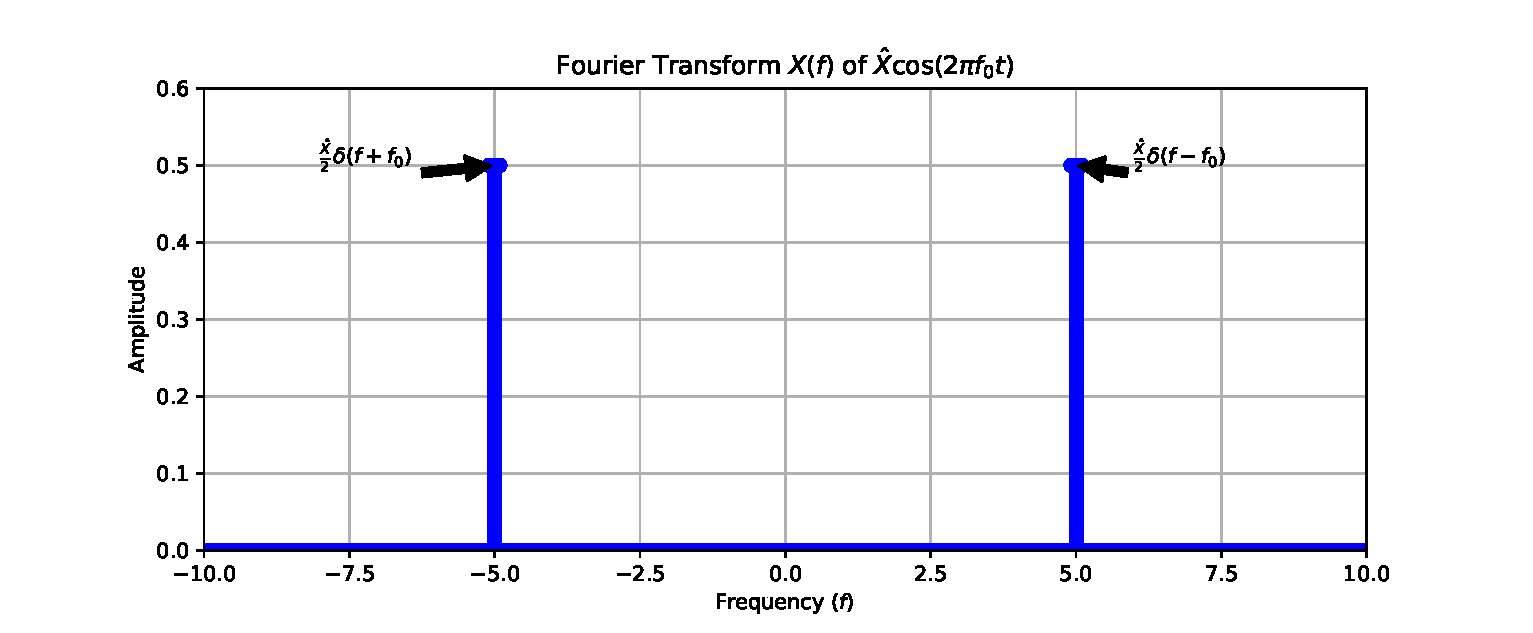
\includegraphics[width=18cm]{ex2_fourier_transformed.eps}
	\vspace{-0.3cm}
	\caption{Fourier Transform.}
	\label{fig:FourierTransform}
	\vspace{-0.1cm}
\end{figure}
